% !TEX root = ..\thesis.tex


\chapter{XÂY DỰNG THIẾT BỊ TỰ ĐỘNG PHÂN LOẠI RÁC}



\section{Xây dựng model phân loại rác dựa trên CNN}



\subsection{Tối ưu model để có thể chạy trên được chip nhúng ESP32}
% phần code 
\begin{figure}[ht]
    \centering
    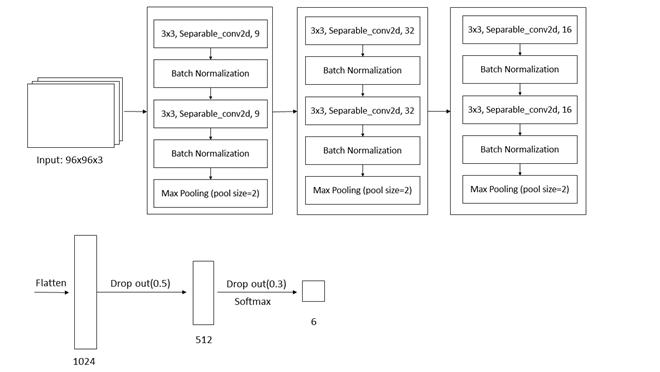
\includegraphics[width=\linewidth]{images/Quanh/ktmang.png}
    \caption{ Minh họa kiến trúc mạng đã xây dựng}
    \label{fig:kientrucmang}
\end{figure}
% QUanhh viết r nè
% Do chip nhúng gì đó chỉ có bao nhiêu ram đó nên chúng tôi không thể xây dựng mô hình với trong số quá lớn và có chi phí tính toán cao được, nên chúng tôi sử dụng ...(thêm đoạn sau vô nè)
% Thêm dụ giảm kích thước của hình ảnh từ bao nhiêu đó xuống 96 * 96 nữa nà

Do sử dụng microcontroller cụ thể là board ESP32 camera AI Thinker, nên ram hỗ trợ rất khiêm tốn. chỉ có 4MB. nên chúng tôi không thể xây dựng mô hình với trọng số quá lớn và có chi phí tính toán cao được. Vì thế, chúng tôi chọn các sử dụng separable convolution thay cho lớp convolution thông thường để giảm bớt chi phí tính toán cho mạng. Ngoài ra ở lớp này, chúng tôi dùng regularization l2 để tránh overfitting và hàm kích hoạt relu – đây là hàm thường được sử dụng trong quá trình train model với dữ liệu dưới dạng ảnh. Chúng tôi cũng thêm các lớp batch normalization và drop out để tránh cho mô hình bị overfitting và loại bỏ sự kết nối chặt chẽ giữa các lớp fully connected. Tổng số tham số của mô hình là 532,161. Sau khi xây dụng mô hình, nhóm đã sử dụng optimization stochastic gradient descent với learning rate = 1e-4 và momentum = 0.8 để train mô hình. Cùng với việc giảm kích thước hình ảnh từ 512 × 384 pixels xuống còn 96x96 pixels để phù hợp với kích thước ram mà board hỗ trợ.

\section{Evaluation}
\subsection{Data Description} % Giới thiệu về dataset ddùng để train và test 
% Dữ liệu được lấy từ cái gì đó quên oy, nhưng cái này nên thêm vô nha
% Kích thước của hình là ... không nhớ a
Chúng tôi dùng bộ dataset TrashNet \cite{trashnet} để train và test với kích thước 512x384.
Gồm 2527 hình thuộc 6 lớp với sự phận bố ở mỗi lớp:
 
Cardboard: 403

Glass: 501

Metal: 410

Paper: 594

Plastic: 482

Trash: 137
 
Dữ liệu được chia làm 2 phần theo tỉ lệ 80\% train và 20\% test.

Train: 2024

Test: 503
Sau đây là hình ảnh minh họa của 6 lớp cần phân loại như trên, bao gồm Cardboard hình \ref{fig:cardboard} , Glass hình \ref{fig:glass}, Metal hình \ref{fig:metal}, Paper hình \ref{fig:paper} , Plastic hình \ref{fig:plastic}, và các loiaj rác thải khác hình \ref{fig:trash}.
\begin{figure}[ht]
    \centering
    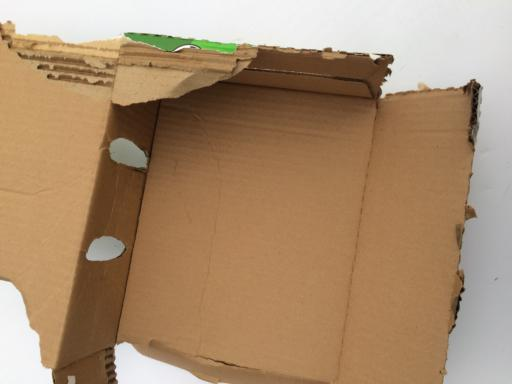
\includegraphics[width=0.25\linewidth]{images/Quanh/cardboard174.jpg}
    \caption{Hình ảnh cardboard trong bộ dataset}
    \label{fig:cardboard}
\end{figure}

\begin{figure}[H]
    \centering
    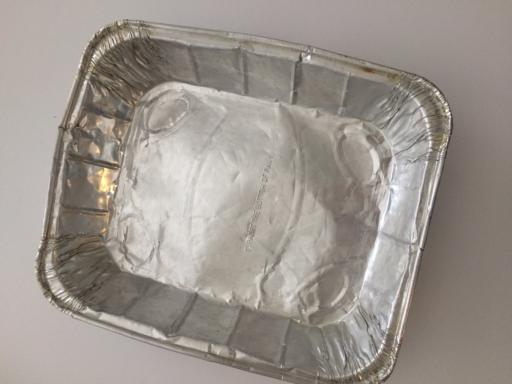
\includegraphics[width=0.25\linewidth]{images/Quanh/metal5.jpg}
    \caption{Hình ảnh metal trong bộ dataset}
    \label{fig:metal}
\end{figure}

\begin{figure}[H]
    \centering
    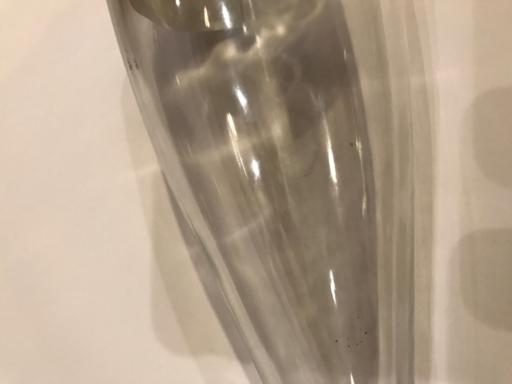
\includegraphics[width=0.25\linewidth]{images/Quanh/glass98.jpg}
    \caption{Hình ảnh glass trong bộ dataset}
    \label{fig:glass}
\end{figure}

\begin{figure}[H]
    \centering
    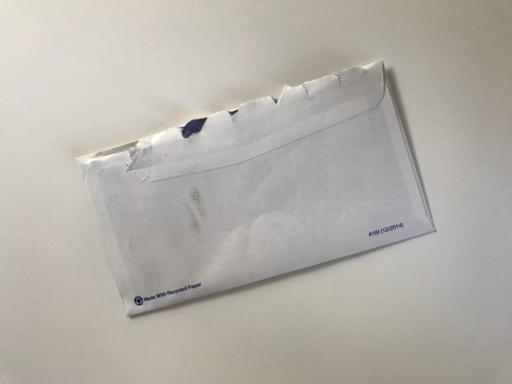
\includegraphics[width=0.25\linewidth]{images/Quanh/paper96.jpg}
    \caption{Hình ảnh paper trong bộ dataset}
    \label{fig:paper}
\end{figure}

\begin{figure}[H]
    \centering
    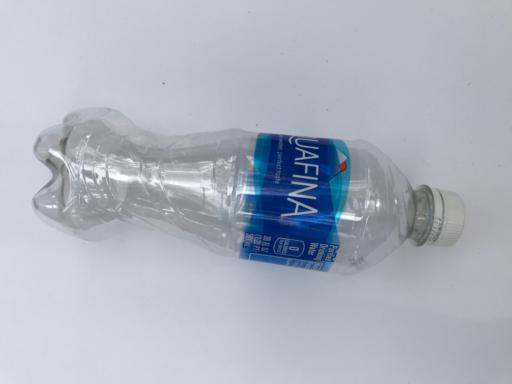
\includegraphics[width=0.25\linewidth]{images/Quanh/plastic49.jpg}
    \caption{Hình ảnh plastic trong bộ dataset}
    \label{fig:plastic}
\end{figure}

\begin{figure}[H]
    \centering
    
\includegraphics[width=0.25\linewidth]{images/Quanh/trash23.jpg}
    \caption{Hình ảnh các loại rác khác trong bộ dataset}
    \label{fig:trash}
\end{figure}
% Nên lựa vài hình về data để thêm vô (nếu cần) hình nên có đủ 6 lớp cần phân loại


\subsection{Index of Performance} % Các chỉ số để dánh gia model  %accuracy, F-score - Recall.
Chúng tôi sử dụng hai chỉ số là accuracy và F1-score để đánh giá model. Accuracy là tính tỉ lệ giữa số ảnh được dự đoán đúng và tổng số ảnh trong tập dữ liệu kiểm thử.
% Còn khúc giới thiệu F1 nữa cơ mà đang lười ghi công thức toán trong đây nha
% Khúc này thêm lý thuyết của hai cái chỉ số đó
\subsection{Kết quả  hiện thực được } % Kết quả  hiện thực được 
Kết quả train mô hình với 80 epoch
\begin{figure}[H]
    \centering
    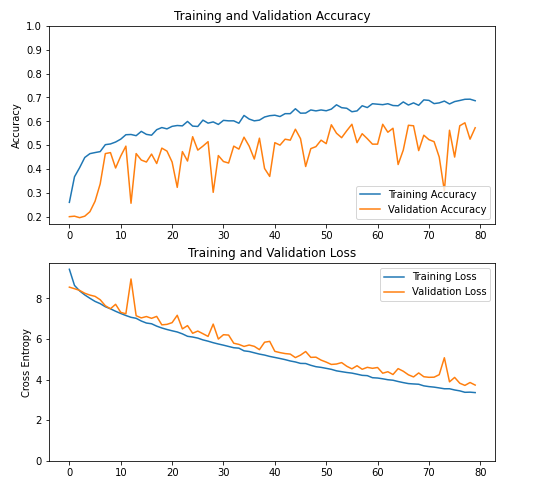
\includegraphics[width=\linewidth]{images/Quanh/graph.png}
    \caption{ Biểu đồ thể hiện loss và accuracy của mô hình trong quá trình train}
    \label{fig:graph}
\end{figure}
% Hai cái này nên chuyển thành dạng bảng, cơ mà đang lười chuyển
Accuracy cao nhất trên tập train là 0.6938 và trên tập test là 0.5938
Loss nhỏ nhất trên tập train là 3.3844 và trên tập test là 3.7116

Kết quả thử nghiệm mô hình trên tập test sau khi đã lưu mô hình tốt nhất từ quá trình train 
\begin{figure}[H]
    \centering
    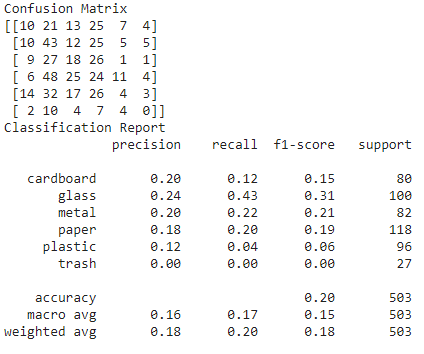
\includegraphics[width=\linewidth]{images/Quanh/matrix.png}
    \caption{ Confusion matrix của model khi thử lại trên tập test}
    \label{fig:matrix}
\end{figure}
Từ hình \ref{fig:matrix} ta có thể thấy accuracy và f1-score của mô hình còn khá thấp, tuy nhiên do mô hình được xây dựng chỉ có 532,161 tham số nên không đủ để phân loại chính xác các lớp được. Chúng tôi đã thử train thêm epoch nhưng mô hình dễ bị overfitting và kết quả khi in confusion matrix vẫn không thay đổi nhiều. Ngoài ra nếu tăng thêm trọng số thì không thể sử dụng model trên thiết bị được.


\section{Build và kiểm thử model phân loại rác trên device}
Sau khi model đã được train và evaluate kỹ lưỡng trên máy tính, công đoạn tiếp theo là build chương trình phân loại rác trên device dựa model đã train và thư viện TensorflowLite. 
Chương tình được build sẽ phải được kiểm thử để đảm bảo khả năng phân loại rác tương đương với khả năng phân loại của model đã được train trên ảnh từ PC.
%\subsection{Quy trình build code phân loại rác trên device}

%Mô tả lại quy trình chuyển đổi từ file h5 của model sang file .cc để đưa vào code
%Đưa vào các đoạn code mẫu của tensorflowLite
\subsection{Kiểm thử chương trình phân loại rác trên device}
%Đưa vào 2 đoạn code C++ và python và mô tả quy trình chạy:
%1. Device start và chờ tín hiệu "bắt đầu chụp ảnh" từ code python trên PC
%2. Mình bấm 1 nút trên PC, code python sẽ gửi tín hiệu "bắt đầu chụp ảnh" qua device
%3. Device chụp ảnh, lưu vào framebuffer của thư viện ESPCam rồi gửi qua cho code Python sau đó chờ tín hiệu "bắt đầu phân loại".
%4. Code python lưu ảnh xuống để thử nghiệm và sau đó gửi tín hiệu "bắt đầu phân loại" cho device.
%5. Device chạy đoạn code phân loại rác của tensorflowLite và gửi kết quả cho code Python sau đó quay lại chờ tín hiệu "bắt đầu chụp ảnh"
%6. Code python hiển thị kết quả phân loại ra cho mình kiểm tra sau đó lưu lại, chờ người dùng nhấn enter để bắt đầu lại quy trình kiểm tra
Để kiểm tra sự phân loại rác sau khi board ESP32 camera AI thinker hoàn thành việc chụp ảnh, tôi sử dụng 1 file python để laptop đóng vai trò như một server để nhận ảnh, detec ảnh, và trả kết quả detec. Việc trao đổi nhận ảnh từ board sang server sẽ sử dụng cable. 

Việc kiểm thử này phải đáp ứng được gần đúng với yêu cầu mà mô hình thực tế hình \ref{fig:chart_smartbin}. Quy trình thực hiện viêc kiểm tra sẽ bao gồm các bước sau:

Khi build file C để nạp code vào board thành công. Tiếp tục build file python để tạo server. Lưu ý vẫn giữ kết nối giữa board và laptop qua cable.

Để thay thế yêu cầu, khi ultrasonic sensor gặp vật cản sau đó khởi động chụp ảnh, thì trong môi trường kiểm tra. Tôi dùng một input được nhập từ bàn phím (nhấn enter) để thay thế bước trên. 
\begin{enumerate}
    \item Nhận input từ người dùng: khi nhấn enter: 
    \item send "1" đến  board.
    \item nhận hình và kết quả dự đoán từ board .
    \item save hình vào local (cùng thư mục vs python, tên file là thời điểm nhận hình).
    \item show kết quả dự đoán trên console và bật app show ảnh ( đã save ở 4)
\end{enumerate}

\subsection{Kết quả phân loại khi chạy trên device}

%Đưa vào vài tấm hình được device chụp và kết quả phân loại tương ứng. 
%Sau đó chém gió là device chạy ra kết quả y chang như model đạt được ở mục trước
Một số hình ảnh được chụp từ thiết bị
\begin{figure}[H]
    \centering
    \includegraphics[width=0.25\linewidth]{images/Quanh/metal.bmp}
    \caption{ Miếng sắt được phân loại vào lớp "Metal" }
    \label{fig:Dmetal}
\end{figure}

\begin{figure}[H]
    \centering
    \includegraphics[width=0.25\linewidth]{images/Quanh/plastic.bmp}
    \caption{ Chai nước nhựa được phân loại vào lớp "Plastic" }
    \label{fig:Dplastic}
\end{figure}

\begin{figure}[H]
    \centering
    \includegraphics[width=0.25\linewidth]{images/Quanh/plastic2.bmp}
    \caption{ Chai nhựa được phân loại vào lớp "Plastic" }
    \label{fig:Dplastic2}
\end{figure}

\begin{figure}[H]
    \centering
    \includegraphics[width=0.25\linewidth]{images/Quanh/cardboard.bmp}
    \caption{ Miếng bìa được phân loại vào lớp "cardboard" }
    \label{fig:Dcardboard}
\end{figure}

\begin{figure}[H]
    \centering
    \includegraphics[width=0.25\linewidth]{images/Quanh/othertrash.bmp}
    \caption{ Các loại rác vò lại méo mó sẽ được phân loại vào lớp "Trash" }
    \label{fig:Dtrash}
\end{figure}

Tuy nhiên, do accuracy của model chỉ ở mức tương đối, và hình ảnh được train và hình ảnh được chụp từ thiết bị sẽ có thay đổi về màu sắc. Nên sẽ có một số loại rác bị detec sai. Dưới đây là các trường hợp sai trong quá trình kiểm thử.
\begin{figure}[H]
    \centering
    \includegraphics[width=0.25\linewidth]{images/Quanh/glass.bmp}
    \caption{ Bao khăn giấy được phân loại vào lớp "glass" }
    \label{fig:DWglass}
\end{figure}

\begin{figure}[H]
    \centering
    \includegraphics[width=0.25\linewidth]{images/Quanh/glassw.bmp}
    \caption{ Vỏ kẹo được phân loại vào lớp "glass" }
    \label{fig:DWglass2}
\end{figure}

\begin{figure}[H]
    \centering
    \includegraphics[width=0.25\linewidth]{images/Quanh/cardboard_W.bmp}
    \caption{ Bàn tay người được phân loại vào lớp "cardboard" }
    \label{fig:DWcardboar}
\end{figure}

Như vậy, tuy có các trường hợp detec sai, nhưng có thể hình dung được mức độ đánh giá của model trong việc detec hình ảnh. Ví dụ như ở hình \ref{fig:DWglass} và \ref{fig:DWglass2}, mặc dù đã bị detec sai lớp, nhưng có thể thấy, thủy tinh nói chung đều có tính chất phản ánh sáng, nên khi hình ảnh khi chụp 1 vật làm bằng thủy tinh sẽ có một độ bóng nhất định. Vì thế ở hình \ref{fig:DWglass} và \ref{fig:DWglass2} đều có tính chất phản ánh sáng như thủy tinh, nên thiết bị sẽ detec vào lớp "glass". Tương tự, các miếng bìa hầu hết trong tập dataset đều có các lằng vân nhấp nhô, và khi thiết bị chụp hình ảnh bàn tay người( hình \ref{fig:DWcardboar}), bàn tay cũng có các đường chỉ tay sâu, nên thiết bị sẽ detec vào lớp "cardboard".


\section{Setup Gateway}
\subsection{Access LG02}
Cấp nguồn điện cho gateway, sau đó dùng laptop để bật scan wifi, lúc này sẽ xuất hiện tên wifi : “dragino-168cb0”

Kết nối với wifi đó và truy cập địa chỉ IP: “10.130.1.1”, lúc này sẽ đến giao diện để configure gateway bằng cách nhập username và password như hình \ref{fig:gateway_configure}
\begin{figure}[H]
    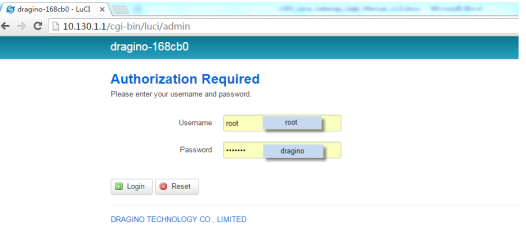
\includegraphics[width=\textwidth]{images/Quanh/Gateway_configure.png}
    \caption{Xác thực tại địa chỉ 10.130.1.1}
    \label{fig:gateway_configure}
\end{figure}

\subsection{Cài đặt network}
Truy cập Internet như Wifi Client theo các bước:
\begin{description}
    \item Bước 1: Network → Wireless, chọn radio0 và scan như hình \ref{fig:radio0_scan}
    \begin{figure}[H]
        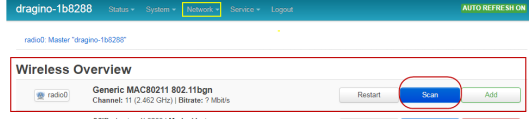
\includegraphics[width=\textwidth]{images/Quanh/Radio_scan.png}
        \caption{Scan mạng Wireless}
        \label{fig:radio0_scan}
    \end{figure}
    
    \item Bước 2: Chọn wifi và tham gia vào mạng, sau đó nhập mật khẩu và Submit như hình \ref{fig:join_password}
    \begin{figure}[H]
        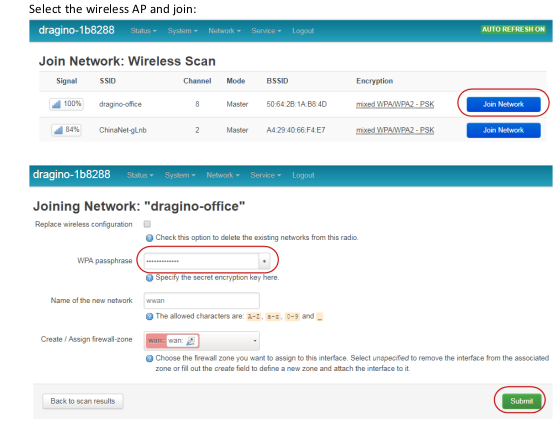
\includegraphics[width=\textwidth]{images/Quanh/Join_password.png}
        \caption{Tham gia vào wifi và nhập mật khẩu}
        \label{fig:join_password}
    \end{figure}
    \item Bước 3: Network → Wireless, chọn disable wifi mặc định của gateway như hình \ref{fig:disable_wifi}
    \begin{figure}[H]
        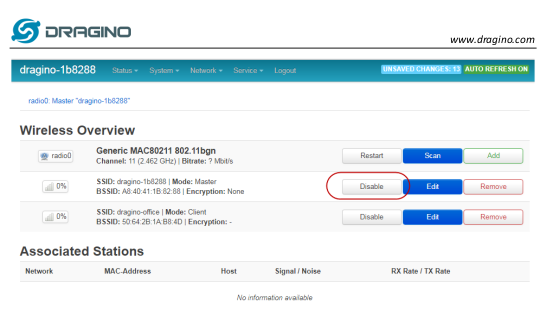
\includegraphics[width=\textwidth]{images/Quanh/Disable_wifi.png}
        \caption{Tắt wifi mặc định}
        \label{fig:disable_wifi}
    \end{figure}
\end{description}
(lưu ý, sau khi thực hiện bước 3, kết nối sẽ bị mất, nếu laptop kết nối wifi mặc định lúc nãy)

Trong trường hợp không thể truy cập địa chỉ 10.130.1.1 nữa, ta sử dụng cổng LAN để kết nối:
\begin{enumerate}
    \item Kết nối LAN Port
    \item Configure Ethernet port có địa chỉ IP như hình \ref{fig:config_ethernet}
    \begin{figure}[H]
        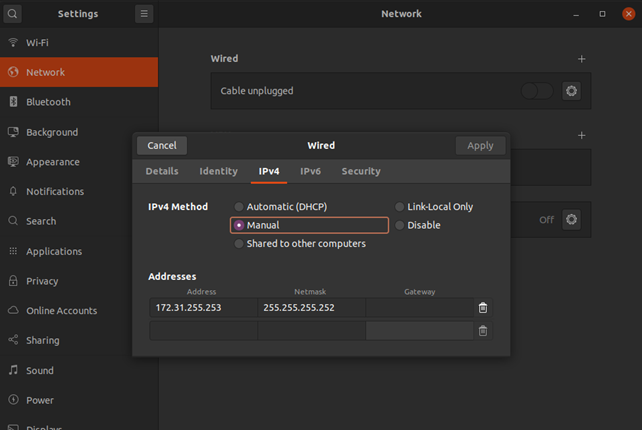
\includegraphics[width=\textwidth]{images/Quanh/Config_ethernet.png}
        \caption{Cấu hình địa chỉ IP của cổng Ethernet (Ubuntu 20.04)}
        \label{fig:config_ethernet}
    \end{figure}
    \item Dùng địa chỉ 172.31.255.254 để truy cập vào Web
\end{enumerate}



\subsection{Tạo gateway trên TTN Server}
\begin{description}
    \item Bước 1: Vào Service → LoRa → Lấy ID của Gateway như hình \ref{fig:get_gateway_id}
    \begin{figure}[H]
        \centering
        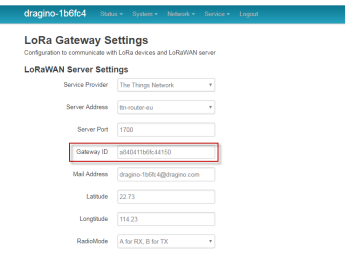
\includegraphics[width=\textwidth]{images/Quanh/Gateway_ID.png}
        \caption{Lấy ID của Gateway}
        \label{fig:get_gateway_id}
    \end{figure}
    \item Bước 2: Truy cập TTN: https://console.thethingsnetwork.org/gateways, giao diện hiển thị ở hình \ref{fig:gateway_console}
    \begin{figure}[H]
        \centering
        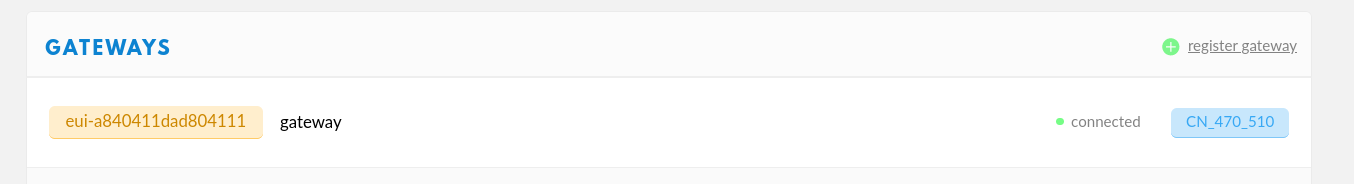
\includegraphics[width=\textwidth]{images/Quanh/Gateway_console.png}
        \caption{Giao diện Gateway đã được tạo (chưa connect)}
        \label{fig:gateway_console}
    \end{figure}
    \item Bước 3: Nhập ID vào Frequency plan tùy thuộc vào Gateway mà chọn cho phù hợp như hình \ref{fig:choose_gateway}, và kết quả được hiển thị ở hình \ref{fig:gateway_result} (nếu power on gateway thì status sẽ hiện "connected")
    \begin{figure}[H]
        \centering
        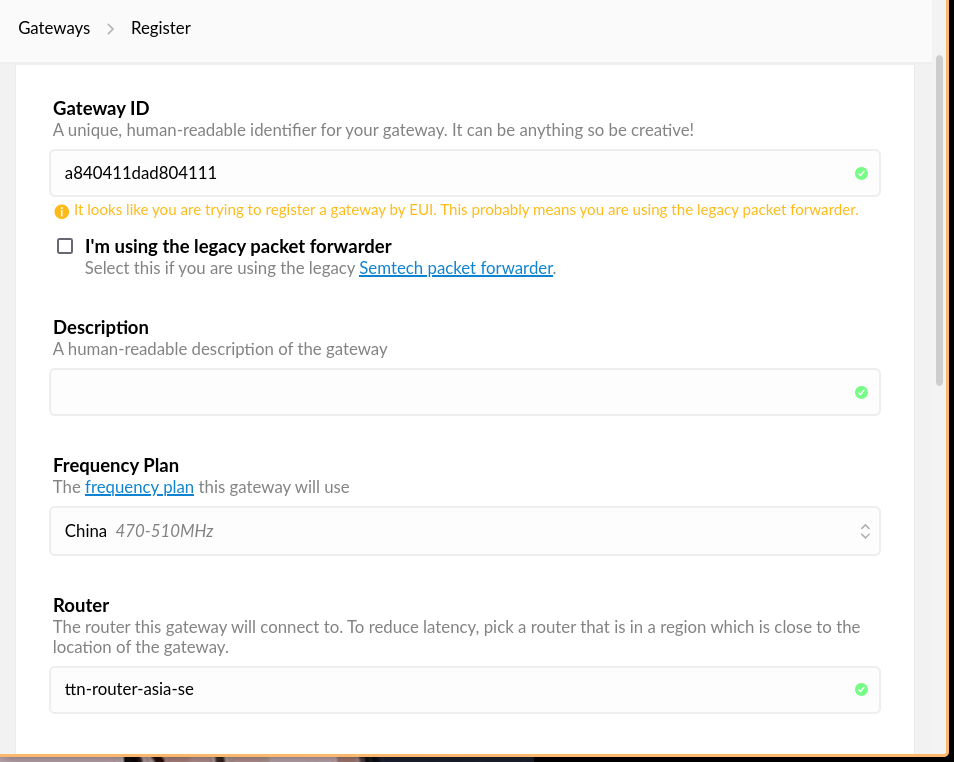
\includegraphics[width=\textwidth]{images/Quanh/Gateway_choose.png}
        \caption{Nhập ID vào Frequency plan}
        \label{fig:choose_gateway}
    \end{figure}
\end{description}
**do Gateway của nhóm sử dụng frequency 433Mhz nhưng The Things Network không hỗ trợ nên khi đăng kí sẽ là : china 470-510Mhz ( do tần số 433 trãi từng tần số 433 đến 510)

\subsection{Configure LG02 Gateway}
\begin{enumerate}
    \item Configure to LoRaWAN server:
    \begin{description}
        \item Bước 1: Config LG02 như hình \ref{fig:config_LG02}
        \begin{figure}[H]
            \centering
            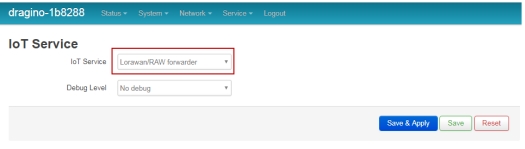
\includegraphics[width=\textwidth]{images/Quanh/Config_lg02.png}
            \caption{Config LG02}
            \label{fig:config_LG02}
        \end{figure}
        \item Bước 2: Chọn server address và gateway ID như hình \ref{fig:choose_server_address} (nhóm chọn ttn-router-asia-se)
        \begin{figure}[H]
            \centering
            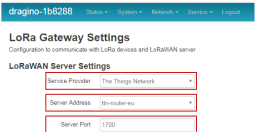
\includegraphics[width=\textwidth]{images/Quanh/Choose_server_address.png}
            \caption{Chọn server address thích hợp}
            \label{fig:choose_server_address}
        \end{figure}
    \end{description}

    \item Configure LG02's RX frequency: Ở frequency 433Mhz, có 8 channel uplink nhưng nhóm chọn channel 433.175Mhz để end-device join vào, thông sô như hình \ref{fig:radio_config}
    \begin{figure}[H]
        \centering
        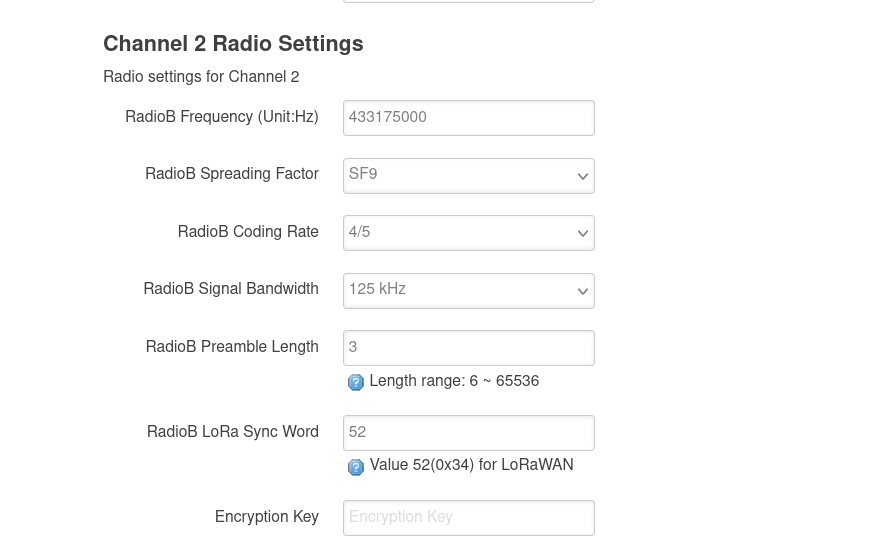
\includegraphics[width=\textwidth]{images/Quanh/Radio_config.png}
        \caption{Thông số configure}
        \label{fig:radio_config}
    \end{figure}
\end{enumerate}


\section{Setup End-Device}
\subsection{Thu gom rác}
Phần mềm sử dụng: Arduino IDE 1.8.2

Ngôn ngữ lập trình: C

Thiết bị Kit RF thu phát wifi Blue esp32 + Lora sx1278 oled Heltec.

\begin{description}
    \item Bước 1: Add lib esp32 từ link https://github.com/HelTecAutomation/Heltec\_ESP32 để thêm thư viện esp32 cho Arduino
    \item Bước 2: Add lib Lmic https://github.com/matthijskooijman/arduino-lmic để thêm vào thư viện Lmic cho Arduino
\end{description}

** Thư viện esp32 hỗ trợ hoạt động trên Heltech ESP32 develop framework.
** Thư viện Lmic cung cấp các giao tiếp LoRaWan ở classA và Class B. Tuy nhiên chỉ hỗ trợ ở band EU-868 và US 915. Nhưng thiết bị nhóm sử dụng là frequency 433Mhz nên cần sửa 1 số file để thiết bị có thể truyền data

Lúc này, có thể nạp code vào board như bình thường.

\subsection{Đăng kí trên TTN Server}
\begin{description}
    \item Bước 1: Tạo Application ID và handler, sau đó vào Devices → Register device → Điền Device ID  
    \item Bước 2: Sau khi đăng kí device thành công, The Things Network sẽ mặc định setup device join vào channel theo OTAA, nhưng nhóm chọn join theo ABP nên cần vào Setting → Activation method → ABP.
    
\end{description}



** ở phần này Payload Formats sẽ tùy thuộc vào code nạp vào end-device



\subsection{So sánh khi sử dụng Cayenne LPP và Custom}

Ta có bảng \ref{tab.comparison.Cayenne}

\begin{table}[H]
    \centering
    \caption{Loại rác} 
    \label{tab.comparison.Cayenne}
    \begin{tabular}{| m{6cm} | m{6cm} |}
        \hline
        Cayenne LLP & Custom \\

        \hline
        •	Không cần decoder (do thư viện Cayenne LPP đã có những quy định về code ở end-device) & •	Cần decoder để TTN hiển thị thông tin \\
        •	Khó hiển thị thêm các trường data từ sensor khác (Vì chỉ  hỗ trợ mặc định cho sensor nhiệt độ độ ẩm, các sensor khác phải qua pin Analog) & •	Có thể thêm nhiều sensor dễ dàng bằng code trên node, và chỉ cần cài đặt Payload formats trên TTN để hiển thị thông tin \\
        •	Mặc định payload & •	Có thể thay đổi Payload \\
        
        \hline
    \end{tabular}
\end{table}

Để chuyển data cho backend, cần cấu hình ở phần Integrations.



\subsection{Lưu ý khi nạp code cho node}

Vì sử dụng phương thức join vào server là ABP nên cần khai báo các thông tin cần thiết vào file *.ino để node có thể send data đến application server 

\begin{itemize}
    \item Device EUI, Network Session key và App Session key
    \item Để tối ưu việc truyền nhận từ node đến gateway,  nên disable các channels không cần thiết( chỉ enable channel đã khai báo ở RX của gateway)
\end{itemize}



